% ------------------------------------------------------------------------------
% TYPO3 CMS 8.1 - What's New (English Version)
%
% @author	Patrick Lobacher <patrick@lobacher.de> and Michael Schams <schams.net>
% @license	Creative Commons BY-NC-SA 3.0
% @link		http://typo3.org/download/release-notes/whats-new/
% @language	English
% ------------------------------------------------------------------------------
% LTXE-CHAPTER-UID:		dcfe6009-2200ad81-816c2edb-1f54c687
% LTXE-CHAPTER-NAME:	Backend User Interface
% ------------------------------------------------------------------------------

\section{Interfaccia utente Backend}
\begin{frame}[fragile]
	\frametitle{Interfaccia utente Backend}

	\begin{center}\huge{Capitolo 1:}\end{center}
	\begin{center}\huge{\color{typo3darkgrey}\textbf{Interfaccia utente Backend}}\end{center}

\end{frame}

% ------------------------------------------------------------------------------
% LTXE-SLIDE-START
% LTXE-SLIDE-UID:		e75a9c1e-b3d6f3ba-5c9edc92-c926d4c0
% LTXE-SLIDE-ORIGIN:	5d3d70fa-92a2935e-f1cbdc1e-285ec842 English
% LTXE-SLIDE-TITLE:		Feature: #75497 - inline backend layout wizard
% LTXE-SLIDE-REFERENCE:	!Feature-75497-InlineBackendLayoutWizard.rst
% ------------------------------------------------------------------------------
\begin{frame}[fragile]
	\frametitle{Interfaccia utente Backend}
	\framesubtitle{Wizard inline per Backend Layout}

	Un nuovo tipo di visualizzazione è stato aggiunto per il wizard del backend layout con il FormEngine in modalità inline
	(in TCA: \texttt{'renderType' => 'belayoutwizard'}).

	\begin{figure}
		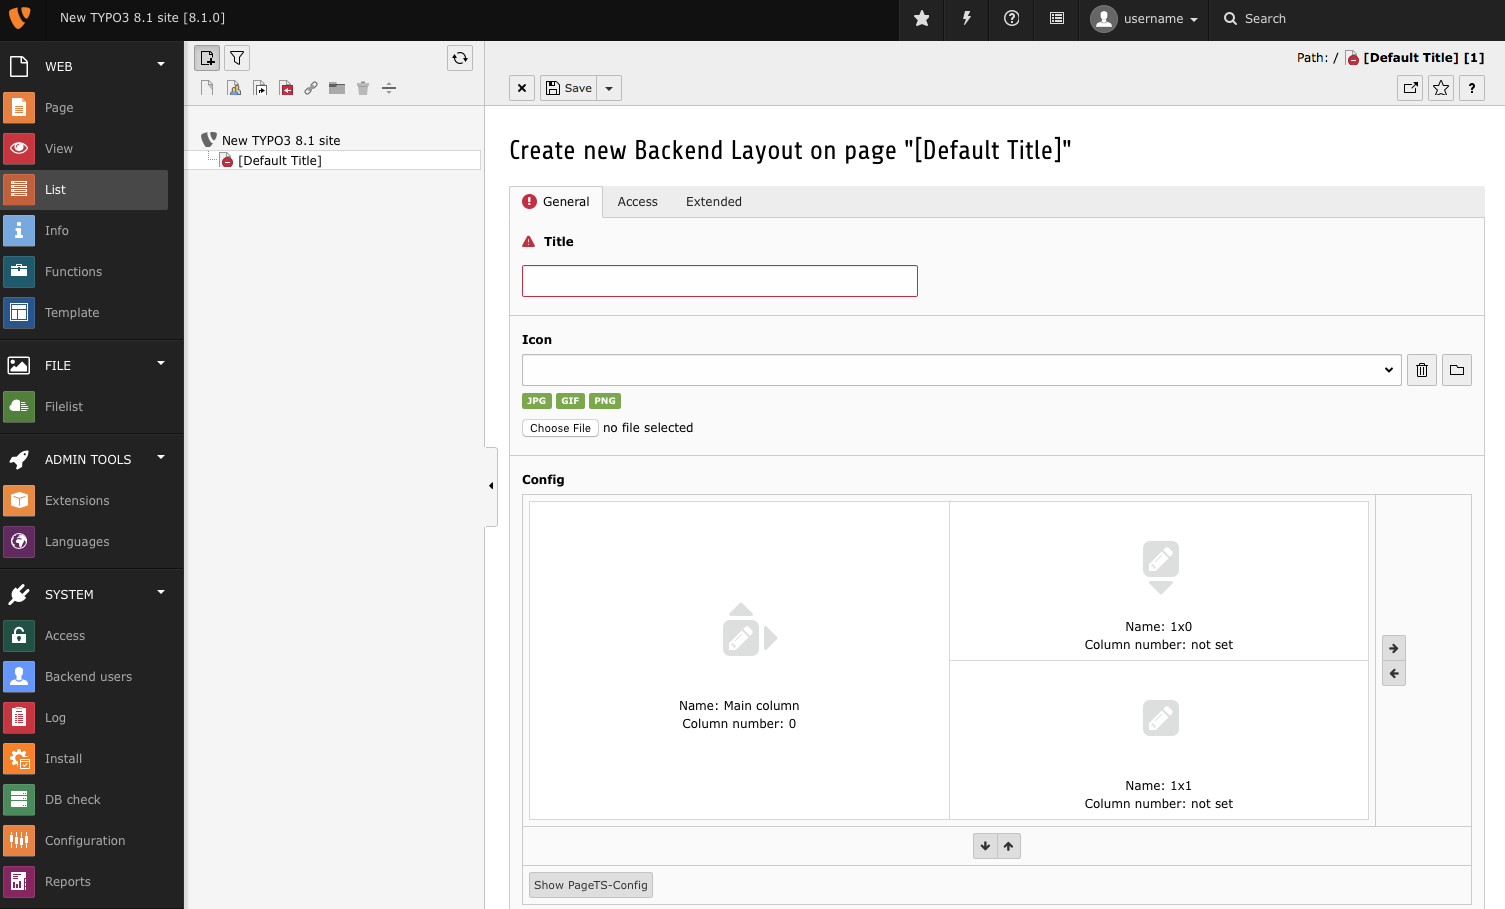
\includegraphics[width=0.70\linewidth]{BackendUserInterface/75497.png}
	\end{figure}

\end{frame}


% ------------------------------------------------------------------------------
% LTXE-SLIDE-START
% LTXE-SLIDE-UID:		7523a331-9206c084-497c0fb9-51417e20
% LTXE-SLIDE-ORIGIN:	7cab4dc0-cdfe9472-a3f0a874-dddf137d English
% LTXE-SLIDE-TITLE:		Feature: #75581 - Simplify cache clearing
% LTXE-SLIDE-REFERENCE:	!Feature-75581-SimplifyCacheClearing.rst
% ------------------------------------------------------------------------------
\begin{frame}[fragile]
	\frametitle{Interfaccia utente Backend}
	\framesubtitle{Semplificazione cancellazione Cache}

	Il sistema di cancellazione della cache è stato semplificato rimuovendo le opzioni nel menu cache clear e
	nell'Install Tool.

	\begin{itemize}

		\item \textbf{Cancellazione della cache di frontend:}\newline
			\small
				Cancellazione della cache di frontend e delle pagine relative, come prima.
			\normalsize

		\item \textbf{Cancellazione di tutte le cache:}\newline
			\small
				Cancellazione di tutte le cache di sistema, incluse le classi di caricamento, le traduzioni,
				file di configurazione delle estensioni e opcode cache. La ricostruzione di queste cache
				può impiegare un po' di tempo.
			\normalsize

	\end{itemize}

	\begin{figure}
		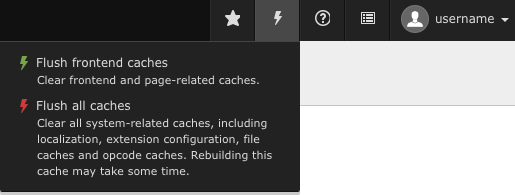
\includegraphics[width=0.45\linewidth]{BackendUserInterface/75581.png}
	\end{figure}

\end{frame}

% ------------------------------------------------------------------------------
% LTXE-SLIDE-START
% LTXE-SLIDE-UID:		e492a526-48bc139b-ef4c924c-1540678e
% LTXE-SLIDE-ORIGIN:	e24e593c-fe9bcff9-c386db3a-79491de1 English
% LTXE-SLIDE-TITLE:		Rework Workspaces (1)
% LTXE-SLIDE-REFERENCE:	Rework Workspaces
% ------------------------------------------------------------------------------
\begin{frame}[fragile]
	\frametitle{Interfaccia utente Backend}
	\framesubtitle{Rielaborazione Workspaces (1)}

	\begin{itemize}

		\item Il modulo di workspace per gestire i contenuti è stato riscritto e
			integrato molto meglio per quanto riguarda l'aspetto visivo nel backend

		\item Gli editori si renderanno conto immediatamente; esso si inserisce nel look generale
			basandosi su Twitter Bootstrap e jQuery

		\item Questo cambiamento porta anche un incremento delle prestazioni ed è un enorme passo
			avanti per un backend di TYPO3 più pulito e veloce con meno javascript.

	\end{itemize}

\end{frame}

% ------------------------------------------------------------------------------
% LTXE-SLIDE-START
% LTXE-SLIDE-UID:		b7dc1c86-39ce811a-ccd559c5-6efbf794
% LTXE-SLIDE-ORIGIN:	fe9bcff9-e24e593c-79491de1-c386db3a English
% LTXE-SLIDE-TITLE:		Rework Workspaces (2)
% LTXE-SLIDE-REFERENCE:	Rework Workspaces
% ------------------------------------------------------------------------------
\begin{frame}[fragile]
	\frametitle{Interfaccia utente Backend}
	\framesubtitle{Rielaborazione Workspaces (2)}

	Immagini del modulo di workspace:

	\begin{figure}
		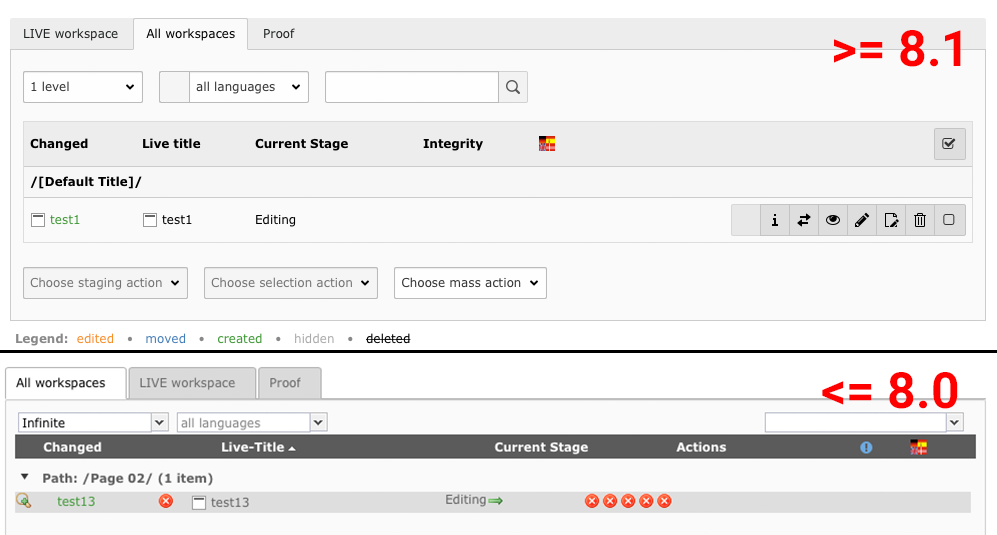
\includegraphics[width=0.85\linewidth]{BackendUserInterface/workspaces.png}
	\end{figure}

\end{frame}

% ------------------------------------------------------------------------------
